% ==============================================================================
\newcommand{\ruta}[1]{\texttt{#1}}
% SECCIÓN 1: INTRODUCCIÓN Y JUSTIFICACIÓN ARQUITECTÓNICA
% ==============================================================================
\section{Diseño de Firmware}

El diseño del firmware para un sistema embebido robótico representa un desafío crítico: se deben ejecutar de manera concurrente tareas de control determinista en tiempo real junto con algoritmos pesados de procesamiento espacial y servicios no deterministas de comunicación inalámbrica.

Para evitar los cuellos de botella característicos de las arquitecturas tradicionales basadas en bucles secuenciales infinitos (\textit{Super-Loops}), se ha seleccionado una \textbf{Arquitectura Jerárquica en Capas} gobernada por el kernel de tiempo real \textbf{FreeRTOS} sobre la plataforma EDU-CIAA.

\subsection{Arquitectura propuesta y criterios de diseño}

El firmware se diseñará para integrar la percepción, la estimación de la pose,
la construcción del mapa y el control del rover diferencial. La arquitectura
será portable entre plataformas: el desarrollo y la validación funcional se
realizarán primero sobre ESP32/Arduino ya que no contamos con una EDU-CIAA en nuestras casas para desarrollar y probar software de aplicación; luego se portará a EDU-CIAA reutilizando la
aplicación y los drivers compartidos, y reemplazando la capa de adaptación al
hardware.

Se adopta una organización en tres capas para separar las operaciones propias
de cada placa de los algoritmos del robot. Esta separación permite probar los
módulos por partes, mantener una única implementación de la lógica del rover y
evitar que las decisiones de una placa condicionen el código común. La
arquitectura de ejecución se organizará en tareas periódicas controladas por
tiempo y planificadas por FreeRTOS, la implementación y caracteristicas de este todavia no se decidieron ya que primero optamos por validar los datos del hardware e integrarlo con una simple versión del scheduler.

El modelo elegido prioriza interfaces estables entre capas, unidades físicas
comunes y un main compartido. El período de muestreo y las prioridades se
ajustarán mediante mediciones de carga y latencia cuando se integren los
encoders, la construcción del mapa y el control de motores.

\newpage
\subsection{Las Tres Capas}

\begin{figure}[h!]
    \centering
    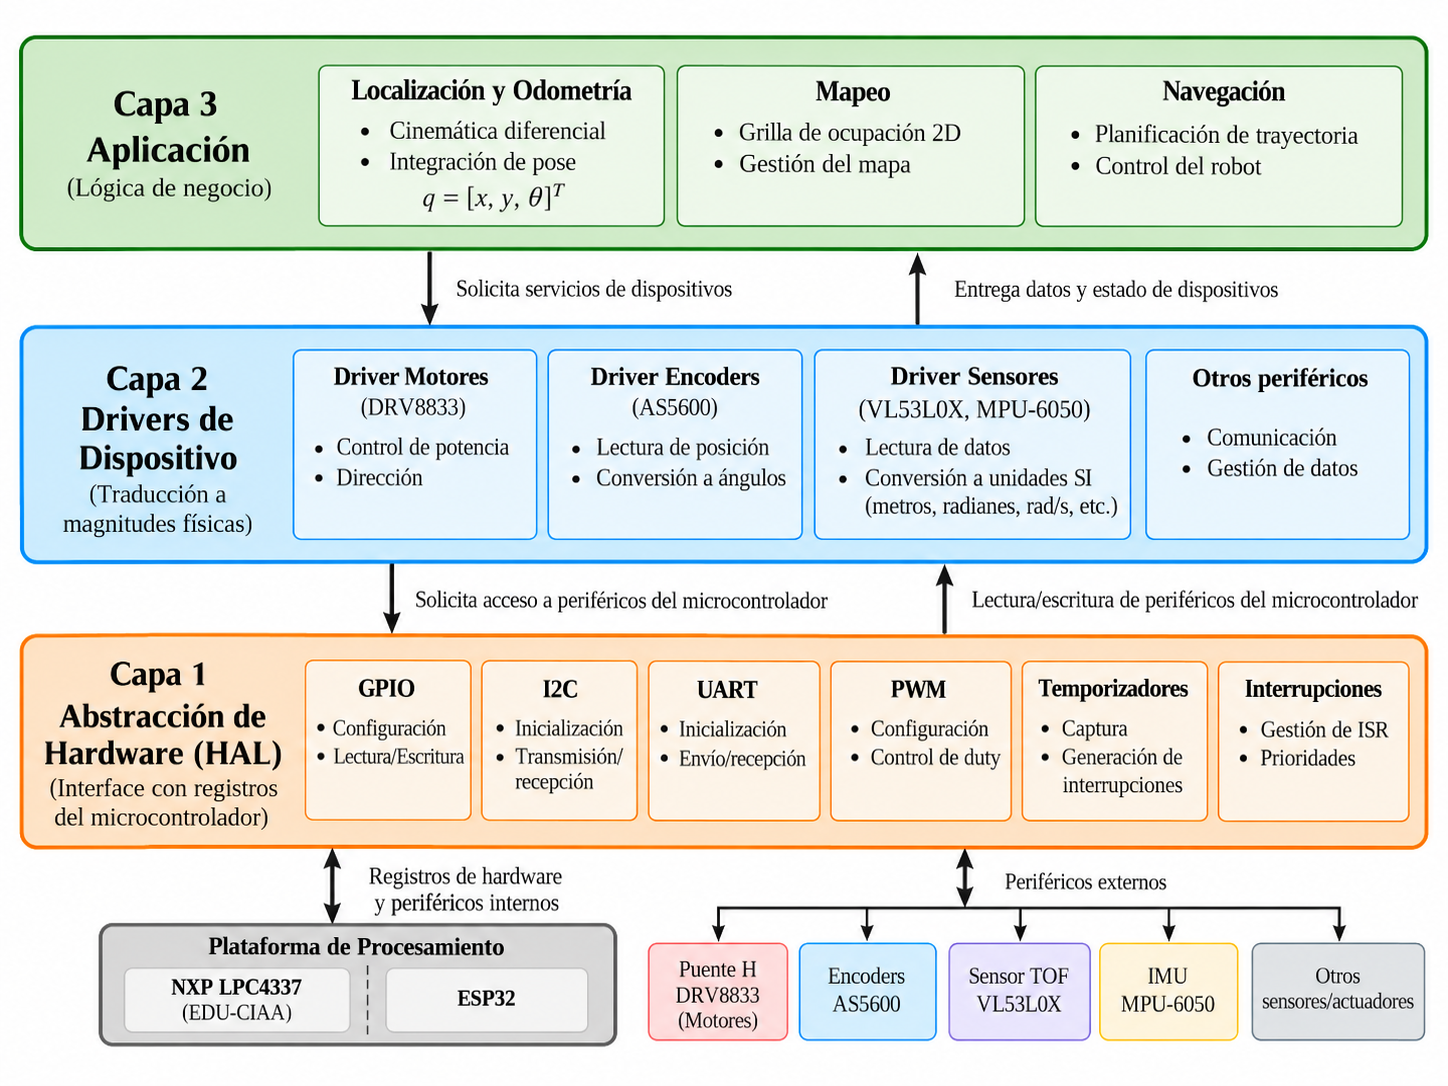
\includegraphics[width=1\textwidth]{capas.png}
    \caption{Estructura jerárquica de la arquitectura en capas para el firmware de Arturito.}
    \label{fig:capas_software}
\end{figure}
\begin{description}

  \item[Capa 1 --- HAL (Hardware Abstraction Layer).]
       Será una interfaz común y tendra una implementación por placa. Su objetivo
        principal es abstraer el acceso a los periféricos y recursos de bajo
        nivel del microcontrolador, tales como GPIO, I2C, UART, PWM,
        temporizadores e interrupciones, evitando que las capas superiores
        dependan directamente de registros o características especificas de
        una arquitectura.

        Cada plataforma tendrá su propia implementación de estas funcionalidades.
        Por ejemplo, una implementación para la EDU-CIAA podrá configurar
        directamente registros del LPC4337, mientras que otra implementación
        podrá utilizar funciones provistas por sAPI o LPCOpen. De manera
        equivalente, una implementación para ESP32 podrá utilizar los drivers
        proporcionados por ESP-IDF.

        Por lo tanto, la existencia de la HAL no implica que todos los
        periféricos deban implementarse desde cero mediante acceso directo a
        registros. Si la arquitectura dispone de una biblioteca o driver que
        ya implementa dicha funcionalidad, la función correspondiente de la
        HAL podrá encapsular esa implementación. De esta manera, las capas
        superiores mantienen siempre la misma interfaz independientemente de
        cómo se resuelva internamente cada operación.

        La HAL no realizará tratamiento de las
        mediciones ni algoritmos propios del funcionamiento del rover.
        Sin embargo, en aquellos casos en que una biblioteca específica de
        una plataforma ya proporcione funciones de mayor nivel para acceder a
        un dispositivo, la HAL podrá encapsular dichas funciones con el fin de
        mantener una interfaz uniforme entre arquitecturas. En estos casos terminaria actuando como una HAL de perifericos.
        El procesamiento
        común de las mediciones continuará perteneciendo a los drivers de
        dispositivos. La HAL tampoco realizará integración de pose, mapeo ni
        navegación.

        \begin{visar}
Ejemplos de funciones HAL:
\begin{itemize}

  \item \texttt{hal\_gpio\_config()} 

  \item \texttt{hal\_gpio\_write()} 

  \item \texttt{hal\_i2c\_init()} 

  \item \texttt{hal\_i2c\_read()} 

  \item \texttt{hal\_pwm\_set\_duty()} 


  \item \texttt{hal\_imu\_get\_gyro\_z\_rads()} representa el caso en que la capa se comporta como HAL de perifericos. Si la plataforma dispone de una
        biblioteca específica para un periferico, podría encapsular directamente
        la función equivalente de dicha biblioteca. De esta forma, las capas
        superiores utilizan la misma interfaz independientemente de la
        implementación disponible en cada arquitectura.

\end{itemize}
        \end{visar}


  \item[Capa 2 --- Drivers de dispositivos.]
        Interpretará las señales físicas de cada dispositivo y entregará datos
        listos para la aplicación. Incluirá lectura, calibración, corrección y
        validación de datos de los sensores y podrá enviar comandos de
        generación de señales de control para el DRV8833. Sus interfaces no
        dependerán de Arduino ni de sAPI.

        \begin{visar}
Ejemplos de funciones de drivers:
\begin{itemize}

  \item \texttt{driver\_mpu6050\_get\_gyro\_z\_rads()}

  \item \texttt{driver\_vl53l0x\_get\_distance\_m()}

  \item \texttt{driver\_as5600\_get\_angle\_rad()} 

  \item \texttt{driver\_motor\_set\_pwm()}

  \item \texttt{driver\_motor\_set\_direction()}

\end{itemize}
        \end{visar}


  \item[Capa 3 --- Aplicación.]
        Contendrá la lógica propia del rover: adquisición y sincronización de
        muestras, cinemática diferencial y estimación de pose, actualización
        de la grilla de ocupación, selección de consignas según el modo y
        distribución de datos a la navegación y las comunicaciones. Acá
        vivirán los algoritmos de estimación de pose, mapeo y navegación.

        \begin{visar}
Ejemplos de funciones de aplicación:
\begin{itemize}

  \item \texttt{odometry\_update()} 



  \item \texttt{pose\_estimator\_update()}

  \item \texttt{occupancy\_grid\_update()} 

  \item \texttt{navigation\_update()} 

\end{itemize}
        \end{visar}


  \item[Infraestructura transversal --- FreeRTOS.]
        FreeRTOS no se considerará una capa adicional de la arquitectura, sino
        una infraestructura transversal utilizada para organizar la ejecución
        concurrente del sistema. El kernel se encargará de la planificación de
        las tareas, sus prioridades y temporización, además de proporcionar
        mecanismos de comunicación y sincronización.

        La lógica de aplicación podrá dividirse en tareas periódicas o
        activadas por eventos, por ejemplo para adquisición de sensores,
        control de velocidad, estimación de pose, actualización del mapa,
        navegación y comunicaciones. Cuando resulte necesario, los drivers y
        la HAL también podrán utilizar mecanismos proporcionados por FreeRTOS
        para sincronizar accesos a recursos compartidos.

        

\end{description}

\subsection{Software de PC e interfaz de usuario prevista}

El alcance para el programa de PC es visualizar la pose del rover y
el mapa actualizado. Para transmitir
pose y mapa sin cable se prevé incorporar Wi-Fi o Bluetooth. La elección entre ambos protocolos queda pendiente. Además desde allí se podran mandar órdenes START/STOP y, como objetivos
secundarios, teleoperación y planificación de rutas; su incorporación como
controles de esta interfaz queda por definir.

\begin{figure}[H]
    \centering
    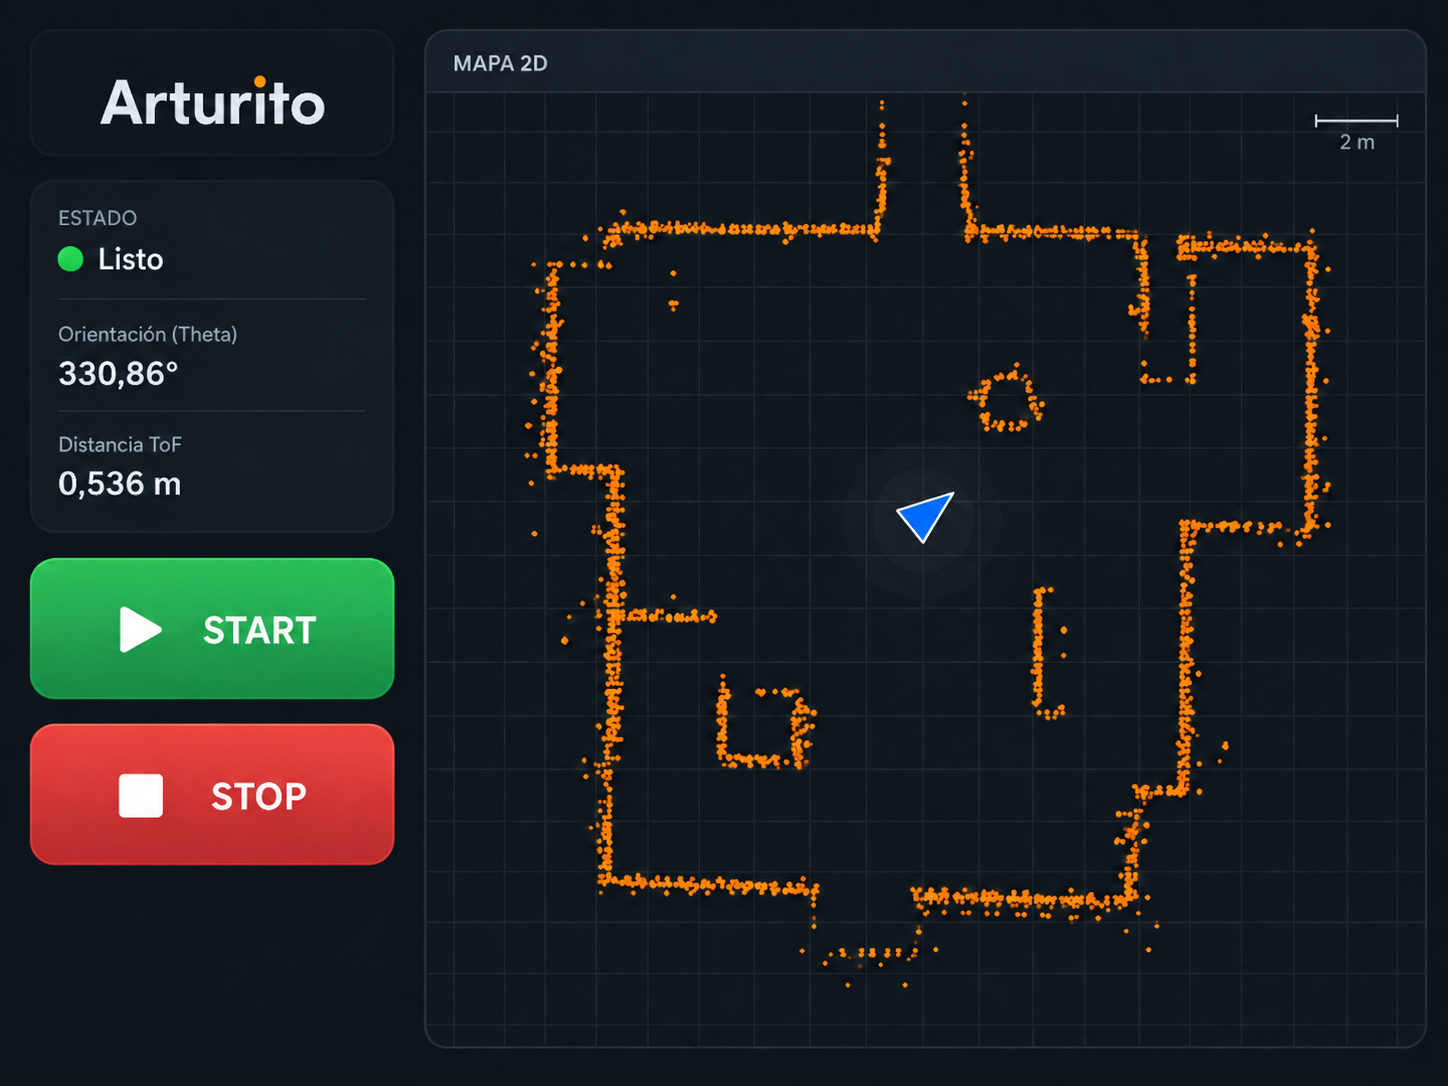
\includegraphics[width=1\linewidth]{InterfazDispExt.png}
    \caption{Interfaz para ver el mapeo desde el punto de vista del usuario.}
    \label{fig:interfaz-dispext}
\end{figure}

Desde esta vista se puede imaginar el siguiente ciclo: 

\begin{center}
\fbox{\parbox{0.91\linewidth}{\centering
Inicio $\rightarrow$ conexión con el rover $\rightarrow$ espera de datos
$\rightarrow$ visualización continua de pose y mapa $\rightarrow$ pérdida de
enlace: indicar desconexión / conexión restablecida: reanudar visualización}}
\end{center}

Si se pierde el enlace durante la operación, el firmware deberá aplicar la
parada segura y la interfaz indicará la desconexión. 

\subsection{Bibliotecas y herramientas externas previstas}

\begin{itemize}
  \item \textbf{ESP32:} framework Arduino y su integración con FreeRTOS;
        \texttt{Wire} para I2C; biblioteca Adafruit \texttt{VL53L0X} para el
        sensor ToF. Para el transporte inalámbrico se utilizará la capacidad
        disponible en ESP32 una vez elegido el protocolo de enlace.
        Para la compilación, carga y estructura general del sistema se utiliza PlatformIO.
  \item \textbf{EDU-CIAA:} LPCOpen y SAPI para la placa y sus periféricos, más
        el kernel FreeRTOS configurado en el proyecto. La HAL de algunos modulos estan implementados (por ejemplo: MPU60x0, el cual brinda acceso simplificado al sensor MPU6050) mientras que hay sensores como el ToF que no tienen esta libreria especifica y al cual le tendremos que desarrollar la implementación de acceso I2C por registros.

  \item \textbf{Workspace:} Se logró integrar ambos entornos de desarrollo en un mismo wokspace para VScode. 

  \begin{figure}[h!]
    \centering
    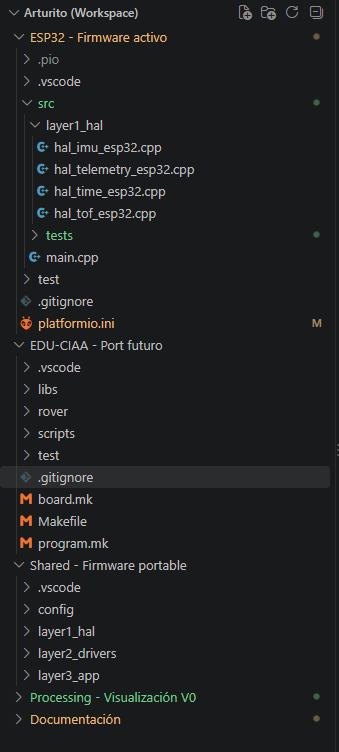
\includegraphics[width=0.3\textwidth]{workspace.png}
    \caption{Estrucura del Workspace.}
    \label{fig:workspace}
\end{figure}
  
  \begin{description}
  \item[\ruta{docs/}] Documentos del equipo.
  \item[\ruta{shared/}] Contratos HAL, drivers y logica de aplicación que no
        deben depender de Arduino ni de sAPI.
  \item[\ruta{esp32/}] Firmware PlatformIO para ESP32, sus HAL de placa y
        programas de diagnostico independientes.
  \item[\ruta{edu-ciaa/}] Copia de estructura del entorno de 'Embedded IDE'. Make, LPCOpen, sAPI, todo lo necesario para la compilación y carga sobre EDU-CIAA. Adapta la
        misma aplicación y drivers a su arquitectura.
  \item[\ruta{processing/}] Por ahora esta carpeta es nuestra "PC externa". Contiene sketches que reciben datos para visualizar.
\end{description}
\end{itemize}


\newpage

\subsection{Estado actual y ensayos realizado}

A la versión actual de firmware la llamamos V0 (Versión 0). Esta versión ya cuenta con la estructura base del workspace explicado anteriormente pero solo realiza el siguiente ciclo de percepción:

\begin{enumerate}
  \item Inicializa la IMU MPU6050 y el sensor de distancia VL53L0X.
  \item Lee la velocidad angular del eje Z de la IMU y una distancia del ToF.
  \item Corrige e integra la velocidad angular para estimar el angulo $\theta$.
  \item Acepta distancias entre 0.05 m y 1.50 m; el resto se representa como
        $-1$ (medida invalida o sensor no disponible).
  \item Publica una linea CSV con $\theta$ en radianes y distancia en metros.
  \item Processing (programa graficador) representa la orientación y acumula puntos del ToF mientras
        el robot gira en el lugar.
\end{enumerate}

No hay todavía odometria XY, encoders, motores, navegación autónoma ni grilla de
ocupación. No hay modos de funcionamiento por comandados ni comunicación inalámbrica.

El firmware V0 fue cargado tanto en ESP32 como en EDU-CIAA y validado con Processing: se comprobó la
recepción de las muestras serie y la visualización de orientación y distancia.
\begin{figure}[h!]
    \centering
    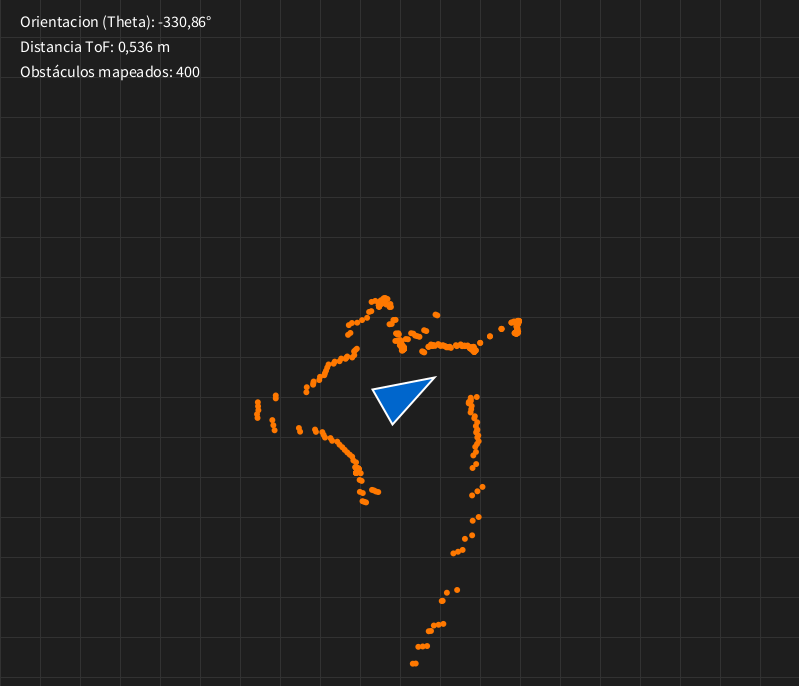
\includegraphics[width=0.6\textwidth]{V0.png}
    \hfill
    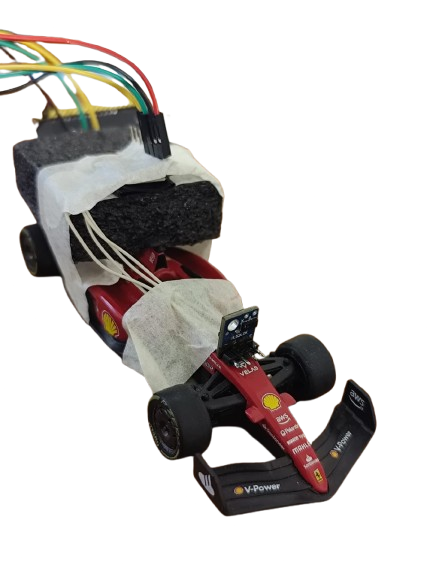
\includegraphics[width=0.38\textwidth]{f1.png}
    \caption{Visualización de V0 en Processing (izquierda) y sensores montados en un auto a control remoto (derecha). \href{https://drive.google.com/file/d/1k8-xx6FHV0KANsshld4rqhePZVvpV37A/view?usp=drive_link}{Link para ver funcionamiento en video.}}
    \label{fig:v0_y_sensores}
\end{figure}

\newpage
\subsubsection{Cómo llegamos a V0}

Firmware V0 es en realidad una versión final de un proceso de testeo de los sensores en ambas arquitecturas, de un proceso de interpretación de datos, de armado de workspace, de ejecución del programa con FreeRTOS, etc.

Algunos cosas interesantes de mensionar:
\begin{description}
 \item[Angulo entregado por capa 1 vs Angulo provisto por capa 2:]
 
 La capa 2 espera que el robot quede quieto, promedia 1000 lecturas separadas por 2
ms para estimar el offset, y reinicia el estado de integración, luego resta el offset, elimina velocidades dentro de ±1◦/s, calcula un promedio trapezoidal entre muestras y acumula el angulo con el tiempo transcurrido.
   \begin{figure}[h!]
    \centering
    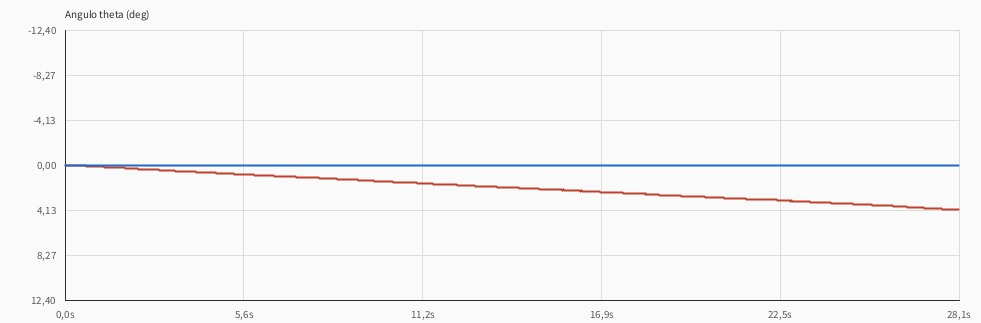
\includegraphics[width=0.9\textwidth]{V0-grados.jpeg}
    \caption{Obtención del angulo crudo vs. procesado por capa 2.}
    \label{fig:grados_crudos}
\end{figure}

Se ve que a tan solo 30s de inicializado el rover el angulo crudo difiere en 5° del angulo real (el rover estaba quieto).

   \begin{figure}[h!]
    \centering
    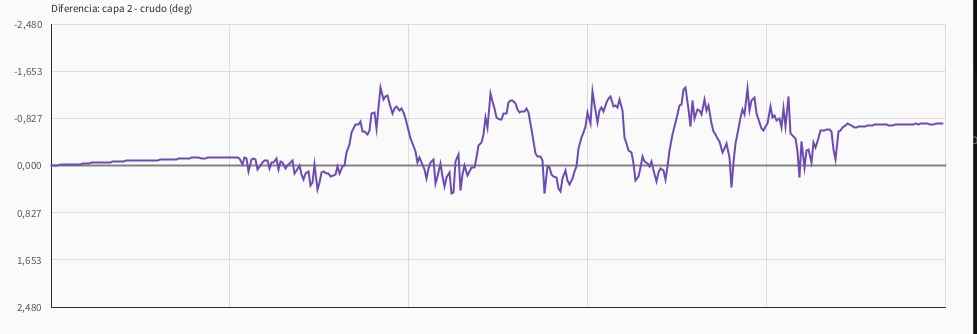
\includegraphics[width=0.9\textwidth]{resta.jpeg}
    \caption{Angulo procesado - Angulo crudo}
    \label{fig:resta_grados}
\end{figure}
Acá se puede ver que si se mueve el robot cambia la relacion entre una señal y la otra. Si el procesado no fuese necesario entonces este grafico deberia ser casi siempre 0 o aunque sea aproximarse a 0. 

 \item[Error en la librería de MPU para EDU-CIAA:] como ya mencionamos, existe una librería que otorga recursos para manejar el giroscopio y acelerometro MPU6050 dentro de sAPI. Durante las pruebas de integración en hardware de se identificó un error que hacia que el sensor no responda.

El procedimiento de arranque de la libreria implementaba una verificación de integridad mediante la lectura del registro interno WHO\_AM\_I (dirección 0x75), cuyo valor de retorno esperado según la hoja de datos estándar del fabricante es 0x68. Sin embargo, la función de inicialización abortaba de forma consistente retornando un código de falla (-5), impidiendo la ejecución del resto del sistema.

Tras analizar el bus de comunicación I2C mediante rutinas de escaneo, se constató que la variante física del módulo utilizado responde con el identificador 0x72 no 0x68. Entendimos que este comportamiento es habitual en hardware genéricos y para solucionar esta incompatibilidad se reestructuró la validación en el driver. La lógica fue modificada para admitir de forma flexible tanto el identificador nativo (0x68) como el valor identificado en el banco de pruebas (0x72).

\end{description}
